% !TEX root =  ../Report.tex

\section{Part 1:  Understanding the methods}
\label{sec:Part 1} 
Now that we have discussed how we will be generating our mazes, we will first discuss the concept behind $A^* search$, and other search methods that exist.


$A^* search$ is an \emph{informed search} strategy. This means that the agent has some knowledge about where the goal state is relative to all other states in the state-space. This is opposed to \emph{uninformed search} strategies, which means the agent is blind about any information for a state, other than the provided problem definition. In other words, this means that an informed search strategy would require information, such as the distance from each state to the goal state, to function properly, where an uninformed search strategy would not need this. The advantage of using an informed search strategy is that the algorithm is much more intelligent and can arrive at the goal in less time as opposed to uninformed search strategies.


This extra information informed search strategies require is often used to feed something called an \emph{evaluation function}, $f(n)$. The definition of $f(n)$ depends on the informed search strategy used, but what we are concerned with is $A^* search$, which has the evaluation function of $f(n) = g(n) + h(n)$, where $h(n)$ is know as our \emph{heuristic function} and $g(n)$ is the cost to reach the current state from our initial state.


As mentioned before, informed search relies on extra information about the states and the goal, and this is where our heuristic function comes into play. $h(n)$ is the distance from each state to the goal state, and it must be \emph{admissible} for $A^* search$ to work properly. This means that $h(n)$ must never overestimate the cost of reaching the goal from state $n$. For any 2 points, an admissible heuristic is often the \emph{euclidean distance} between the 2 points, which is just the straight line distance. For our mazes, since we are operating on a grid world with only 4 main compass directions, we will use something called \emph{Manhattan distances}, which is defined as the sum of the absolute difference between 2 coordinates. The reason this is admissible for our mazes is that the Manhattan distance is the absolute shortest path for any 2 cells in our maze, and it will almost always be an underestimate since the shortest path is likely blocked by a wall somewhere.


\begin{figure}[ht]
  \centering
  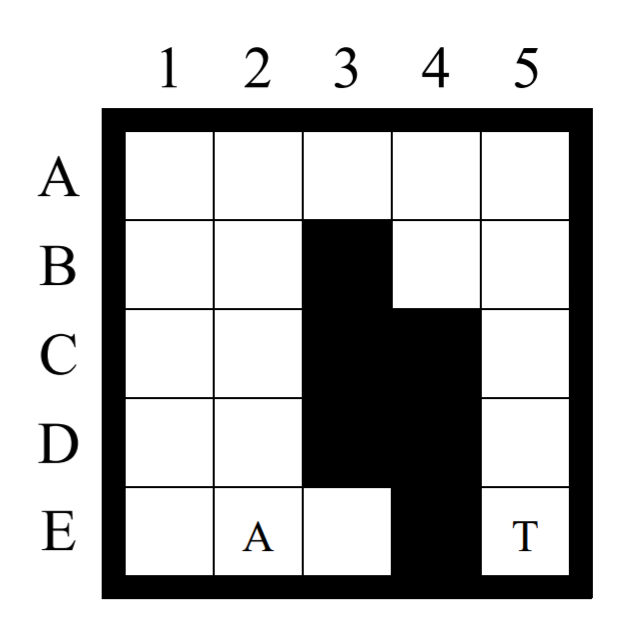
\includegraphics[width=0.35\linewidth]{Report/Part1/maze.PNG}  
\caption{Sample maze problem}
\label{samplemaze}
\end{figure}

In \emph{figure \ref{samplemaze}} we can see a small sample maze. Our initial state is cell \emph{E2} and our goal state is \emph{E5}. Our agent does not initially know about the walls so we will walk through what happens that causes the agent to first move to cell \emph{E3}.
\begin{enumerate}
  \item Begin in \emph{E2} and check for walls. No adjacent walls exist, so perform $A^* search$
    \begin{itemize}
    \item Add E2 to open list
    \item Remove node in open list with lowest f-value (E2) and add to closed list. Then add neighbors to open list
        \begin{itemize}
            \item Cell E3: g(n) = 1, h(n) = 2, f(n) = 3 
            \item Cell D2: g(n) = 1, h(n) = 4, f(n) = 5 
            \item Cell E1: g(n) = 1, h(n) = 4, f(n) = 5 
        \end{itemize}
        \item Remove node in open list with lowest f-value (E3) and add to closed list. Then add neighbors to open list. (We do not add a node that is in the closed list)
        \begin{itemize}
            \item Cell E4: g(n) = 2, h(n) = 1, f(n) = 3 
            \item Cell D3: g(n) = 2, h(n) = 3, f(n) = 5
            \item Cell D2: g(n) = 1, h(n) = 4, f(n) = 5 
            \item Cell E1: g(n) = 1, h(n) = 4, f(n) = 5 
        \end{itemize}
        \item Remove node in open list with lowest f-value (E4) and add to closed list. Then add neighbors to open list.
        \begin{itemize}
            \item Cell E5: g(n) = 3, h(n) = 0, f(n) = 3
            \item Cell D4: g(n) = 3, h(n) = 2, f(n) = 5
            \item Cell D3: g(n) = 2, h(n) = 3, f(n) = 5
            \item Cell D2: g(n) = 1, h(n) = 4, f(n) = 5 
            \item Cell E1: g(n) = 1, h(n) = 4, f(n) = 5
        \end{itemize}
        \item Remove node in open list with lowest f-value (E5) and this is our goal node. $A^* search$ is now complete, and has returned the path: $E2 \longrightarrow E3 \longrightarrow E4 \longrightarrow E5$
    \end{itemize}
    \item Now we move along this path to E3, and realize a wall exists in our path (E4). We then perform another \emph{$A^*$ search}.
\end{enumerate}
The above walk through demonstrates why our agent will move east as its first action. It is inherently because the agent cannot observe the walls that are in its way until it is adjacent to the walls. This causes the \emph{$A^*$ search} to find the optimal path without considering the blockage.


It is important to note that in searching these finite grid worlds, we are guaranteed to either find a solution if it exists. And if a solution does not exist, we know that this is the case. The reason behind this is that all cells in our grid world are connected, with some being walls. We can think of these walls as discontinuations in the grid. Because of this, any location in our grid that is not an island can be reached in some form or another through a linked list of cells travelled. On the other hand, any islands that exist cannot be reached from other islands. This is very analogous to the earth, if we assume water represents our walls in the grid. We can technically get to any point on a connected piece of land by car, but not so if the land is surrounded by water. This is automatically implemented in \emph{$A^*$ search} since any nodes in our open list can be traced to the initial start node. After all nodes are in the closed list, our open list becomes empty  and the goal is not reached, we know that no solution exists. And this can be done in finite time since our grid world is finite to begin with.

We can also analyze the maximum number of cells an agent would travel before it reaches its goal or finds out it cannot reach the goal. Take the same 5 X 5 grid in \emph{figure \ref{samplemaze}}. We will prove the following:


\begin{qoute}
\emph{Prove that the number of moves of the agent until it reaches the target or discovers that this is impossible is bounded from above by the number of unblocked cells squared.}
\end{qoute}
\begin{proof}
Let $S$ be the set of all cells in the grid, with $|S| = 25$ and $B$ be the set of all unblocked cells for the known environment, where $|B| = 19$. By using $A^* search$, we will be adding each expanded node to the closed list, meaning for node x, $\forall x \in closedList:$ $x \notin openList$. Therefore, the set of all moves, $X$, has the property that $|X| \leq |B|$.


This shows that for a known environment, the number of moves the agent can explore until it reaches the goal cannot be greater than the state space. However, we are dealing with an initially unknown environment.We must therefore expand this definition for \emph{repeated forward/backward $A^* search$}. The pseudo code of this is shown below:

\begin{algorithm}
    \caption{Repeated forward/backward $A^* search$}
    \begin{algorithmic}
    
    \STATE $current = start$
    \STATE $path \leftarrow computeAstar(current)$
    \WHILE{$current \neq goal$}
    \STATE $walls \leftarrow update()$
    \IF{$path.next \neq wall$}
        \STATE $current \leftarrow path.next$
    \ELSE
        \STATE $path \leftarrow computeAstar(current, walls)$
        \IF{$path == NULL$}
            \RETURN{"No Path Exists!"}
        \ENDIF
    \ENDIF
    \ENDWHILE
    \end{algorithmic}
\end{algorithm}

We can observe that \emph{Repeated forward/backward $A^* search$} has the only difference with the fact that it calls $A^* search$ every time it encounters a new obstacle on its current path. Therefore, since each $A^* search$ is bounded by $|X| \leq |B|$, where $X$ is the set of all nodes explored by $A^* search$ and $B$ is the set of all open cells on the grid, we can also infer that $A^* search$ will not be called on nodes that have already been travelled, since we have a static environment. Therefore, for the set of travelled nodes, $Z$, we have $|Z| \leq |X|*m$, where $m$ is the amount of times $A^* search$ is called. And we know from before, that $m \leq |X|$. We can assume a worst case situation and have $m = |X|$. Finally, by substitution we obtain $|Z| \leq |X|^2$ and the upper bound of this with substitution would be $|Z| \leq |B|^2$.

\end{proof}